\documentclass[10pt]{beamer}

\usetheme[progressbar=frametitle]{metropolis}
\usepackage{appendixnumberbeamer}

\makeatletter
\setlength{\metropolis@progressinheadfoot@linewidth}{3pt}
\makeatother
\usepackage{caption}
\usepackage{subcaption}


\setbeamercolor{background canvas}{bg=white}
\usepackage{booktabs}
\usepackage[scale=2]{ccicons}
\usepackage{adjustbox}
\usepackage[makeroom]{cancel}
\newcommand\Ccancel[2][black]{\renewcommand\CancelColor{\color{#1}}\xcancel{#2}}

\usepackage{pgfplots}
\usepackage{multirow}
\usepgfplotslibrary{dateplot}

% COLORS
\usepackage{xcolor}
\definecolor{kured}{RGB}{144, 26, 30}
\definecolor{kugrey}{RGB}{102, 102, 102}
\definecolor{kudarkgrey}{RGB}{35, 55, 59}
\definecolor{steelblue4}{RGB}{54, 100, 139}
\definecolor{brown1}{RGB}{255, 64, 64}
\definecolor{mix}{RGB}{155, 82, 102}

% FIGURES 
\usepackage{float}
\usepackage{tikz}

% SHOW LATEX
\usepackage{listings}
\lstset
{
    language=[LaTeX]TeX,
    breaklines=true,
    basicstyle=\tt\scriptsize,
    keywordstyle=\color{blue},
    identifierstyle=\color{magenta},
}

% REFERENCES
\usepackage[authoryear]{natbib}
\bibliographystyle{apalike}
\renewcommand{\bibsection}{}

% GRAPHICS
\graphicspath{{figures/}}

\usepackage{xspace}
\newcommand{\themename}{\textbf{\textsc{metropolis}}\xspace}

\usepackage[sfdefault]{FiraSans} %% option 'sfdefault' activates Fira Sans as the default text font

\definecolor{kured}{RGB}{144, 26, 30}
\definecolor{kugrey}{RGB}{102, 102, 102}
\usecolortheme[named=kured]{structure}
\setbeamercolor{title separator}{fg = kured, bg = kugrey}
\setbeamercolor{progress bar}{fg = kured, bg = kugrey}
\metroset{block=fill}
\title{Introduction to \LaTeX}
\subtitle{Overleaf, Beamer, and Github}
\author{Carl-Emil Pless, PhD Student}
\institute{Department of Food and Resource Economics \\ The University of Copenhagen}
\titlegraphic{\hfill\includegraphics[height=1.5cm]{KUlogo.pdf}}
\date{8th of October 2021}


\begin{document}

\maketitle

\begin{frame}{Introduction to \LaTeX}
    \emph{All material is available \href{https://github.com/carlepless/latex-introduction}{\color{blue}here} . Please contact me at \href{mailto: cep@ifro.ku.dk}{\color{blue}cep@ifro.ku.dk} if you have any additional questions or comments.} 
    \tableofcontents    
\end{frame}

\section{Introduction}

\subsection{Getting started}
\begin{frame}{Getting started}
    \alert{Let's start by creating an \texttt{Overleaf} account:}
    \begin{enumerate}
        \item Please go to: \href{https://www.overleaf.com/edu/ucph}{\color{blue}https://www.overleaf.com/edu/ucph}
        \begin{itemize}
            \item Make an account using your KUmail 
            \item This claims a professional version (with room for more projects, room for more collaborators, synchronization with \texttt{github}, track changes features, and more...)
        \end{itemize}
        \item Then, create a new project by pressing the big green button!
    \end{enumerate} 
\end{frame}

\subsection{What is \LaTeX?}
\begin{frame}{What is \LaTeX?}
\begin{itemize}
    \item \LaTeX is a document processor that unlike MS Word is not a \emph{\alert{what you see is what you get}} program 
    \item A wide variety of \LaTeX \:processors exist: VS Code, Scientific Workplace, MikTeX, LyX, and so on\dots 
    \item \alert{Overleaf} is just one such processor, with some useful built-in features:
    \begin{itemize}
        \item Like Google Docs, you can collaborate with others (just better, and prettier)!
        \item Auto-complete features, dictionaries, de-buggers, and \alert{track-changes}
    \end{itemize}
\end{itemize}
\end{frame}

\begin{frame}[fragile]{What is \LaTeX?}
    The same slide as \alert{before}, but now un-compiled:
\begin{lstlisting}
    \begin{itemize}
        \item \LaTeX is a document processor that unlike MS Word is not a \emph{\alert{what you see is what you get}} program 
        \item A wide variety of \LaTeX \:processors exist: VS Code, Scientific Workplace, MikTeX, LyX, and so on\dots 
        \item \alert{Overleaf} is just one such processor, with some useful built-in features:
        \begin{itemize}
            \item Like Google Docs, you can collaborate with others (just better, and prettier)!
            \item Auto-complete features, dictionaries, de-buggers, and \alert{track-changes}
        \end{itemize}
    \end{itemize}
\end{lstlisting}
\end{frame}

\section{Your first project}
\subsection{About coding...}
\begin{frame}{About coding...}
    A few \alert{remarks on coding} (in general) and \LaTeX:
    \begin{itemize}
        \item Google like there is no tomorrow!         
        \item Remember that time spent \alert{coding up something cool} is never wasted. You can always reuse it later in other projects. 
    \end{itemize}
\end{frame}

\begin{frame}{About coding...}
    A few \alert{remarks on coding} (in general) and \LaTeX:
    \begin{itemize}
        \item Google like there is no tomorrow! 
        \item Remember that time spent \alert{coding up something cool} is never wasted. You can always reuse it later in other projects. 
        \item Find yourself some useful resources:
    \end{itemize}
    \begin{figure}
        \centering 
        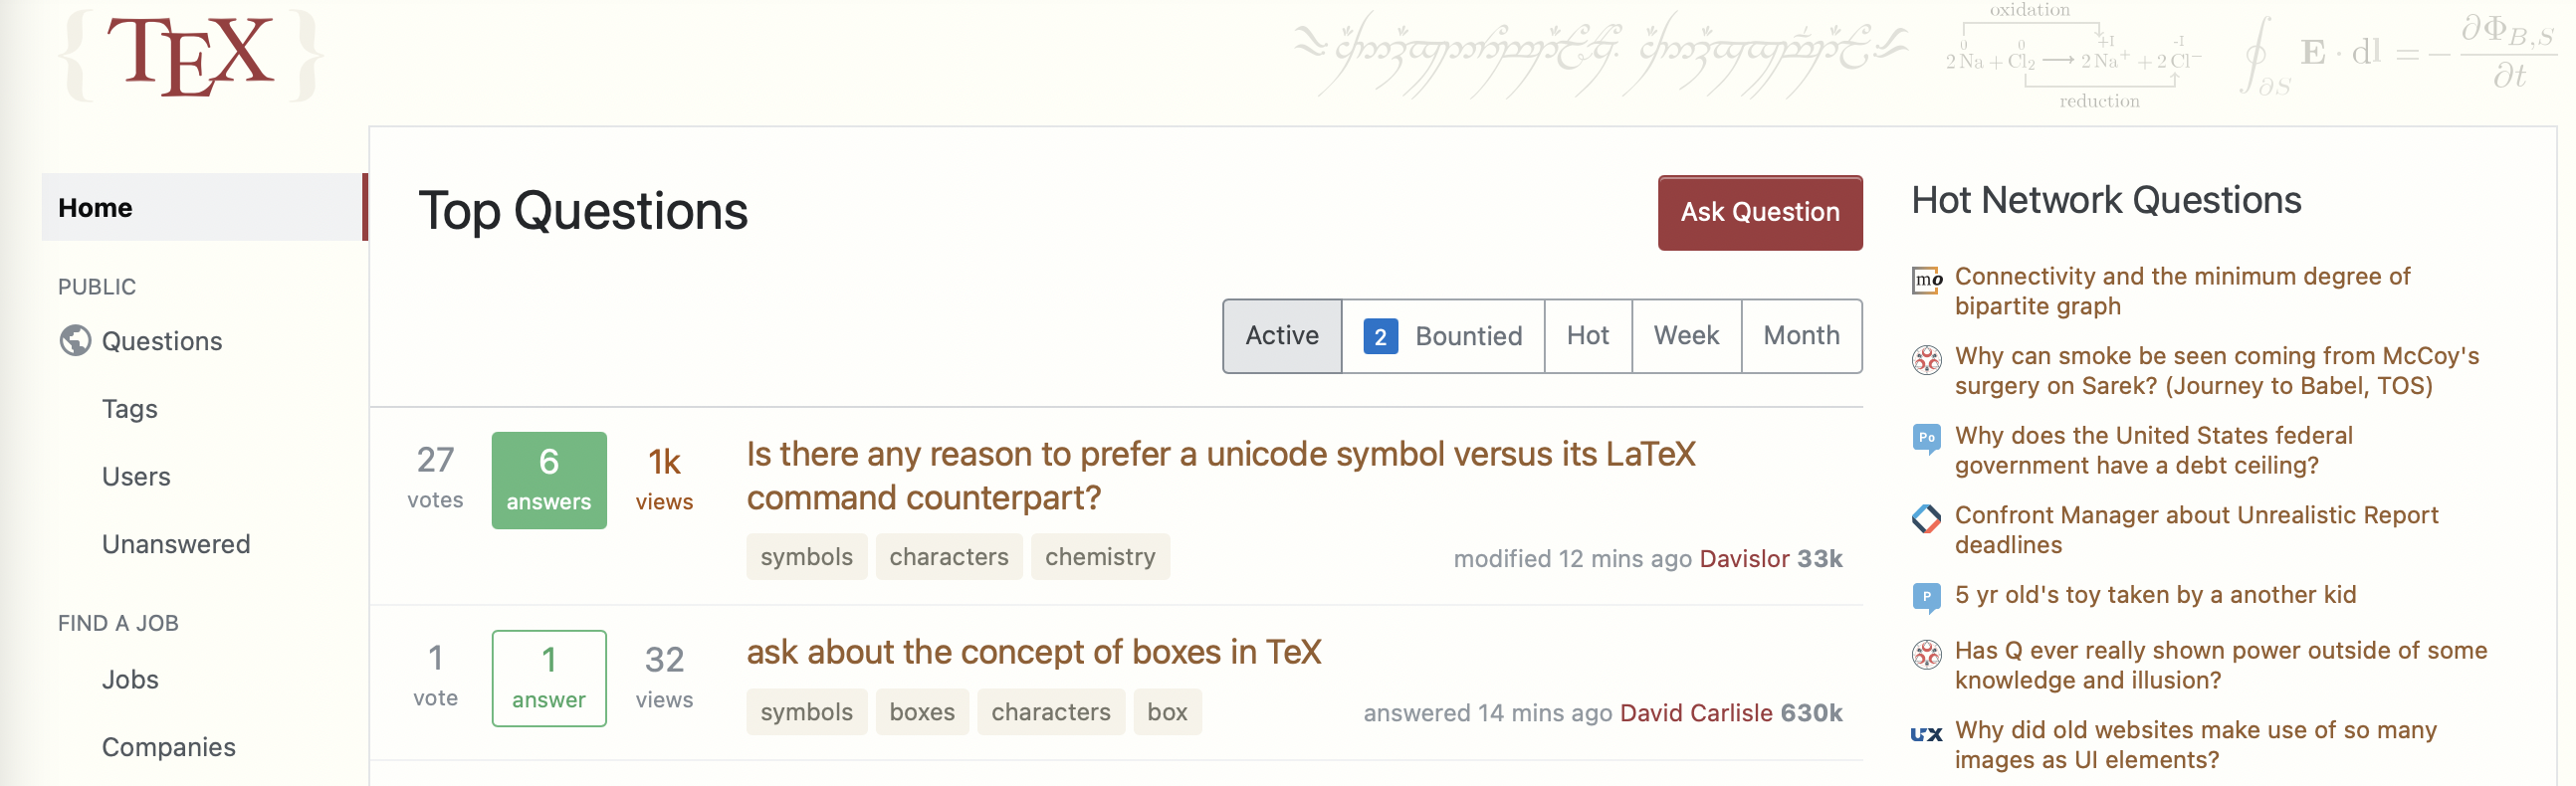
\includegraphics[width = \textwidth]{stackexchange.png}
    \end{figure} 
\end{frame}

\begin{frame}{Intended Learning Outcomes}
    After this session you should... 
\begin{itemize}
    \item<2-> Be \alert{familiar} with the basic syntax and workings of \LaTeX
    \item<3-> Understand the principles of the \alert{preamble} and \alert{BibTeX}
    \item<4-> Be comfortable with using \alert{using Overleaf} for your next larger assignment or project 
    \item<5-> Be able to recreate \alert{most (if not all)} of today's \href{https://github.com/carlepless/latex-introduction/blob/main/cheat-sheet/cheat-sheet.tex}{\color{blue}cheat sheet}
\end{itemize}
\end{frame}

\subsection{Tips and tricks}
\begin{frame}[fragile]{Tips and tricks}
    A few things to note: 
    \begin{enumerate}
        \item<2-> \LaTeX \: is \alert{case sensitive}:
        \item<3-> Some characters serve \alert{specific purposes}:
        \begin{itemize}
            \item<4-> For instance, the percentage sign (\%) is used for commenting and has to be exited with a backslash (\textbackslash) 
            \item <5-> ... and backslash has to be written as \lstinline{\backslash}
        \end{itemize}
        \item<6-> Remember to end your environments:
        \begin{lstlisting}
            \begin{align*}
                y = \alpha + \beta x + u
            \end{align*}   
        \end{lstlisting}
        \item<7-> And proper parenthesis placement:
        \begin{lstlisting}
            \frac{1}{x_{1}^{2}}
        \end{lstlisting}
    \end{enumerate}
\end{frame}

\begin{frame}[fragile]{Tips and tricks}
    \textbf{Writing math}: 
    \begin{itemize}
        \item This is where \LaTeX \: \alert{excels}
        \item<2-> When including math in your \emph{inline} text you just have to wrap it in \$ signs:
        \onslide<3->\begin{lstlisting}
            $ "insert math here" $
        \end{lstlisting}
        \item<4-> Naming is \alert{fairly intuitive} (and identical to writing math in MS Word)
        \item<5-> If you want to center an equation, you can use the \texttt{align*} environment 
        \onslide<5-> \begin{lstlisting}
            \begin{align*}
                y = \alpha + \beta x + u
            \end{align*}    
        \end{lstlisting}
        \item<6-> Note that the \alert{asterisk (*)} determines whether or not it should be numbered    
    \end{itemize}
\end{frame}

\subsection{Get typing!}
\begin{frame}{Using Overleaf}
\textbf{Plan:}
\begin{itemize}
    \item We are going to generate \href{https://github.com/carlepless/latex-introduction/blob/main/cheat-sheet/cheat-sheet.pdf}{\color{blue}this document} step-by-step
    \item Or you can choose to work on some ongoing project or an upcoming assignment
\end{itemize}
A couple of things to \alert{remember}:
\begin{itemize}
    \item Make use of the many online sources of help
    \item Reuse your previous \alert{code}!
    \item There is an \alert{almost infinite} number of solutions to any problem - use the one that makes the most sense for you
\end{itemize}
\onslide<2-> \alert{Start by going to:} \href{https://github.com/carlepless/latex-introduction}{\color{blue}https://github.com/carlepless/latex-introduction} and have a look at the first two sections in \texttt{cheat-sheet.pdf}.
\end{frame}

\section{cheat-sheet.Rtex (.pdf)}
\section*{R and Overleaf}
\begin{frame}[fragile]{R and Overleaf}
    Corresponds to \alert{section 3} in \texttt{cheat-sheet.pdf}:
    \begin{itemize}
        \item All you need to do in order to \alert{compile R directly} in Overleaf is to change the name of the document to \texttt{.Rtex}:
        \onslide<2->\begin{lstlisting}
            <<>>=
            the_answer = function(x){sqrt(x)}
            to_everything = 42^2
            the_answer(to_everything)
            @
        \end{lstlisting}
        \item<3-> Which naturally will return \alert{42}
        \item<4-> Try playing around with replicating some stuff from \texttt{cheat-sheet.pdf} (or your own project)
    \end{itemize}
\end{frame}

\section*{Making tables and inserting figures}
\begin{frame}{Making tables and inserting figures}
    An important \alert{warning}...
    \begin{itemize}
        \item<2-> Making tables in \LaTeX \: is an advanced form of self-torture
        \item<3-> Therefore, the goal is to minimize time spent manually making tables and \alert{maximize automatization}
        \item<4-> For regression tables, use the \texttt{stargazer} package
        \item<5-> If you want to make manual adjustments, use resources like \href{https://www.tablesgenerator.com}{\color{blue}https://www.tablesgenerator.com}, which can convert \texttt{.txt} to \texttt{.tex}
    \end{itemize}
\end{frame}

\begin{frame}[fragile]{Making tables and inserting figures}
    But sometimes, you just can't curb your enthusiasm and simply must make a table:
        \begin{center}
        \begin{lstlisting}
            \begin{table}[H]
                \centering
                \caption{My very first \LaTeX \: table}
                \label{tab:my_label}
                \begin{tabular}{c|c|c}
                    Variable & Description & Type  \\ \hline
                    \texttt{wage} & Wage in USD per hour & Numeric  \\
                    \texttt{educ} & Years of education & Integer \\
                    $\vdots$ & $\vdots$ & $\vdots$ \\
                    $\vdots$ & $\vdots$ & $\vdots$ \\
                    \texttt{married} & Marital status & Binary\\
                    \hline \hline 
                \end{tabular}
            \end{table}
        \end{lstlisting}
        \end{center}
    \end{frame}

\begin{frame}[fragile]{Making tables and inserting figures}
    \begin{table}[H]
        \centering
        \caption{My very first \LaTeX \: table}
        \label{tab:my_label}
        \begin{tabular}{c|c|c}
            Variable & Description & Type  \\ \hline
            \texttt{wage} & Wage in USD per hour & Numeric  \\
            \texttt{educ} & Years of education & Integer \\
            $\vdots$ & $\vdots$ & $\vdots$ \\
            $\vdots$ & $\vdots$ & $\vdots$ \\
            \texttt{married} & Marital status & Binary\\
            \hline \hline 
        \end{tabular}
    \end{table}
\end{frame}

\begin{frame}[fragile]{Making tables and inserting figures}
    \begin{itemize}
        \item Inserting figures on the other hand, is \alert{pretty straightforward}
    \begin{center}
        \begin{lstlisting}
            \begin{figure}[H]
                \centering
                \caption{My nice figure}
                \label{fig:my_label}
                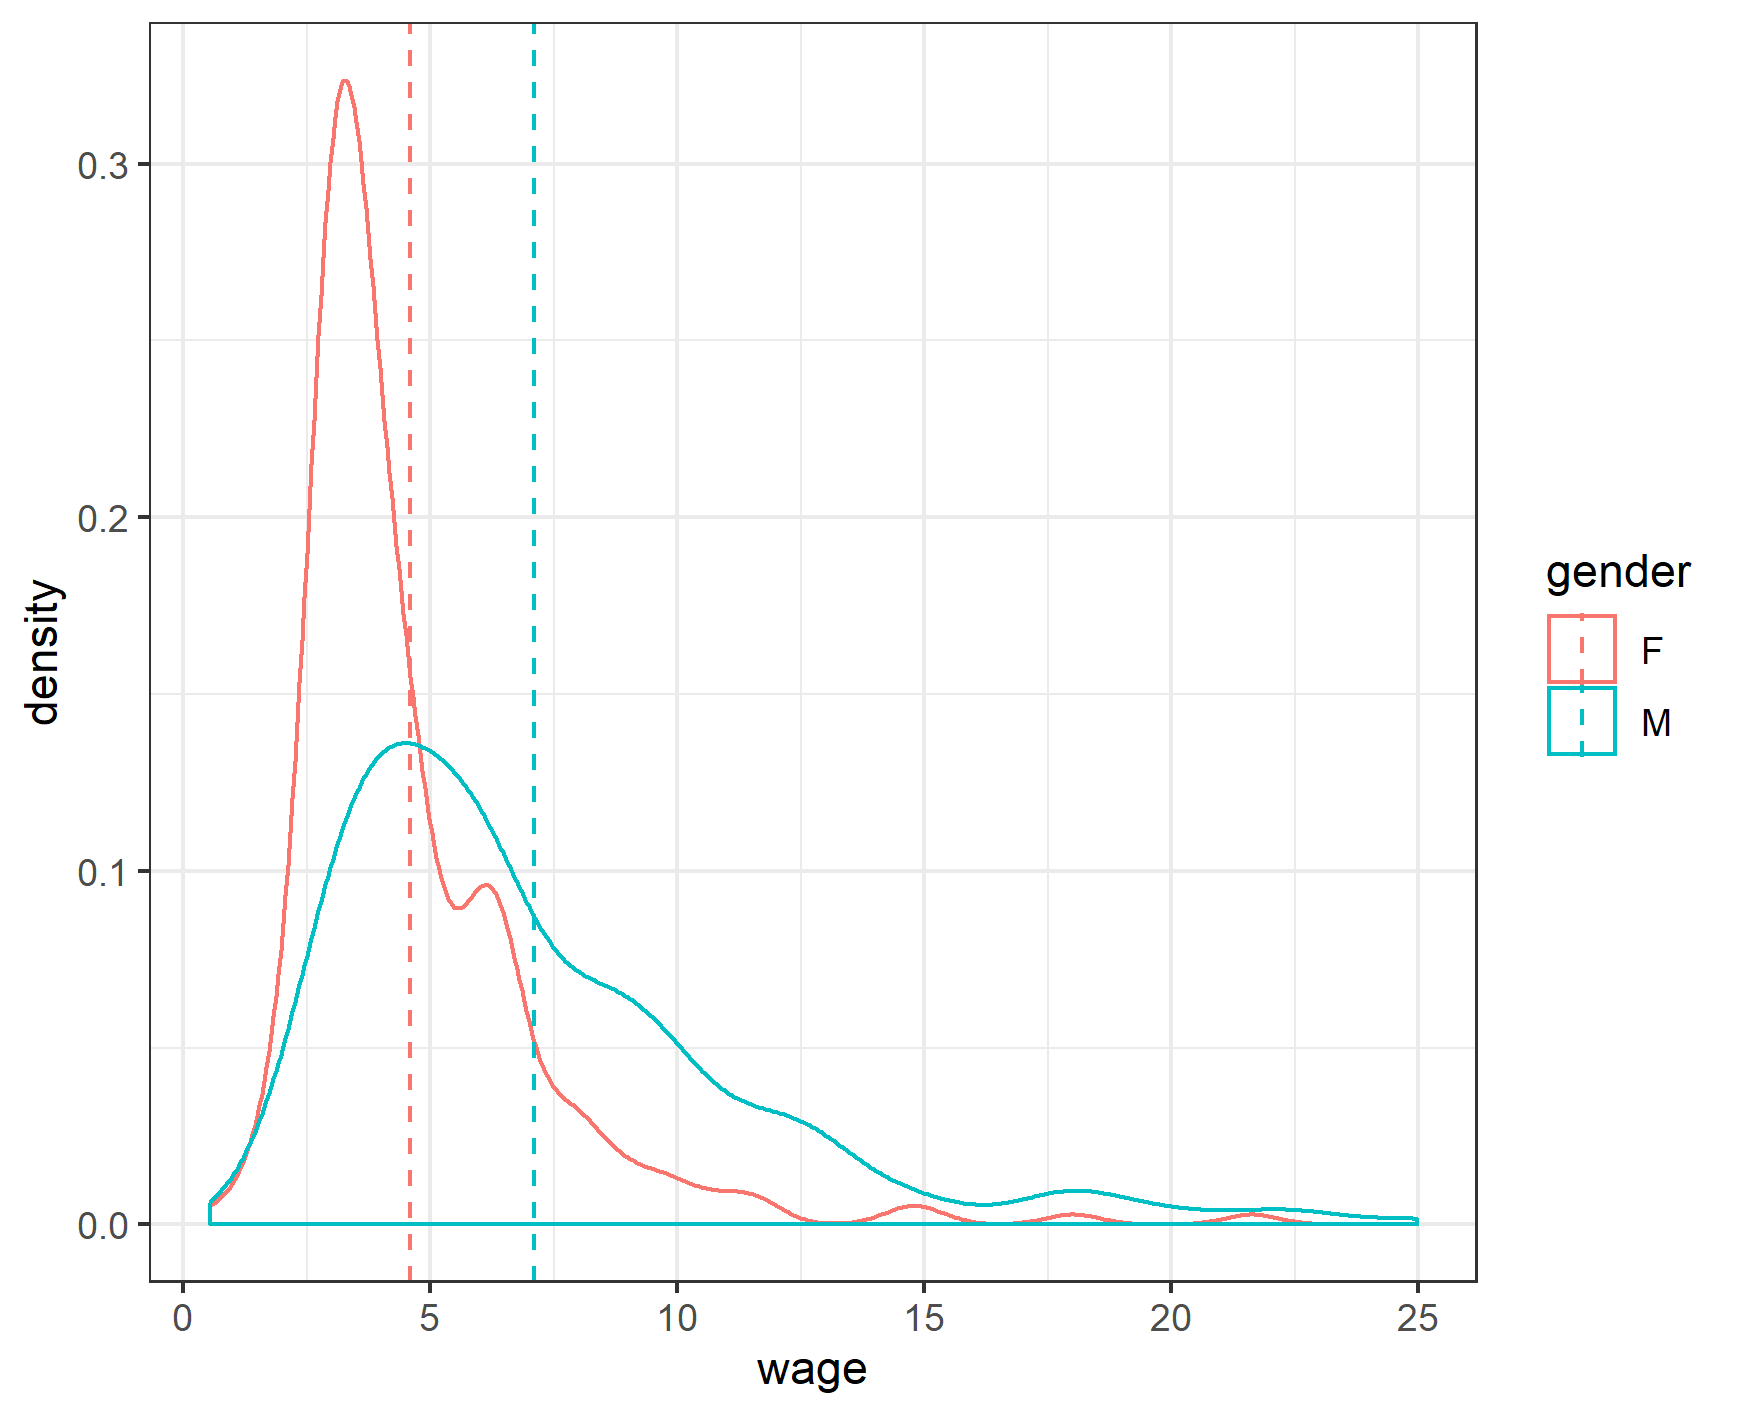
\includegraphics[width=\textwidth]{plot.png}
            \end{figure}
        \end{lstlisting}
        \end{center}
        \item Here, you can scale using the \lstinline{width = } command
        \item Remember that the \lstinline{[H]} determines the placement
        \item<2-> Try playing around with \alert{section 4.1 and 4.2}
        \item<3-> If you are familiar with regression tables, you can also look at \alert{section 5} on \texttt{stargazer}     
    \end{itemize}
\end{frame}

\section*{BibTeX}
\begin{frame}[fragile]{BibTeX: Reference management}
    \begin{itemize}
        \item BibTeX is a bibliography system made specifically for \LaTeX
        \item It seems intimidating and is a bit clunky at first, but it \alert{always} ensures proper reference management (if used correctly)
    \end{itemize}
    \onslide<2->Essentially, you specify an entry as:
    \begin{lstlisting}
        @Book{Verbeek2017,
                title     = {A Guide to Modern Econometrics},
                publisher = {John Wiley \& Sons},
                year      = {2017},
                author    = {Verbeek, M.},
                address   = {Rotterdam School of Management, Erasmus University, Rotterdam},
                edition   = {Fifth},
                }
    \end{lstlisting}
    \begin{itemize}
        \item<3-> Which you can then cite actively with \lstinline[language = tex]!\cite{Verbeek2017}! and passively with \lstinline[language = tex]!\citep{Verbeek2017}!
        \item<3-> As long as Verbeek2017 is an entry in your \texttt{.bib} file 
    \end{itemize}
\end{frame}

\begin{frame}[fragile]{BibTeX: Reference management}
\begin{itemize}
    \item For more information, check out \alert{section 6} in \texttt{cheat-sheet.pdf} 
\end{itemize}
\onslide<2-> In practice, use a reference management program! 
\begin{itemize}
    \item<2-> Zotero, Mendeley or similar
    \item<3-> In both, you can import a BibTeX entry directly and then \alert{export all your references} to a \texttt{.bib} file that you can upload to Overleaf   
\end{itemize}
\end{frame}

\section*{More advanced topics}
\begin{frame}{More advanced topics}
    There are a lot of \alert{neat extensions} to \LaTeX, \: some examples include:
    \begin{enumerate}
        \item \texttt{tikz}
        \begin{itemize}
            \item A package that allows you to draw pixel perfect graphs, illustrations, and figures with complete customizability
            \item I included a couple of examples in the \texttt{cheat-sheet.pdf} but otherwise I recommend looking at \href{https://sites.google.com/site/kochiuyu/Tikz}{\color{blue}TikZ Cookbok}
        \end{itemize}
        \item \texttt{beamer}
        \begin{itemize}
            \item An extension that allows you to create slides (like PowerPoint) with \LaTeX
            \item Has the same advantages (and disadvantages)
            \item Extremely useful if you need to give a presentation that is very math or code intensive 
            \item Feel free to use my theme for this  \href{https://github.com/carlepless/latex-introduction/blob/main/presentation/presentation.tex}{\color{blue}presentation}
        \end{itemize}
    \end{enumerate}
\end{frame}

\end{document}